\pdfminorversion=4
\documentclass[hidelinks]{report}

\usepackage{graphicx}
\usepackage{times}
\usepackage{plain}
\usepackage[plainpages=false]{hyperref}
\usepackage{courier}
\usepackage{caption}

% To force figures to appear after text(along with [H] option)
\usepackage{float}

% To apply linespacing to some content
\usepackage{setspace}

% To show commands, code snippets
\usepackage{listings}

% To use checkmark (tick symbol)
\usepackage{amssymb}

\graphicspath{ {images/pdf/} }

\pagestyle{plain}

\fontfamily{Times}
\selectfont

\setlength{\textwidth}{6.5in}
\setlength{\textheight}{8.5in}
\setlength{\topmargin}{-0.25in}
\setlength{\oddsidemargin}{-0.00in}
\setlength{\evensidemargin}{-0.00in}

% To use multirow feature of latex tables
\usepackage{multirow}

% Using and defining own color
\usepackage{color}
\definecolor{mycol}{RGB}{52, 43, 41}

% Defining courier font usage syntax
\newcommand{\cf}[1] {
	\textbf{\texttt{#1}}
}

% Defining checkmark usage syntax
\newcommand{\T} {
	\checkmark
}

\begin{document}
%% Line spacing 1.5 applied
\setstretch{1.5}

\chapter*{vEPC 2.0 Developer Manual}
In this manual we majorly deal with the process converting our vEPC 1.0 to a distributed design. We describe the distributed architecture of vEPC 2.0 and discuss the strategies used to achieve them.


\paragraph*{NOTE:}

 Please go through Developer manual in vEPC 1.0 to know about I) Design and implementation details of various software modules that were developed as part of v1.0 II) A high level description of individual source code files (\cf{.cpp/.h}). Please read the \cf{user\_manual\_2.0.pdf} under \cf{doc} folder for instructions on experimenting with  vEPC 2.0.
 
\section*{Overview of vEPC 2.0}
Here we present our distributed LTE EPC with horizontal scaling capabilities, state preservation and fault tolerance. We introduce a load-balancer in front of EPC VNFs to maintain a single point of interface with other entities. We keep a number of worker replicas as back-end servers while internally enabling capabilities of adding more back-end servers with increasing load to ensure horizontal scalability. Our design overcomes the state loss problem by keeping states in a reliable data store outside the VNF component. The VNF states can be synced to the data store at three different granularity (i) Always sync: where transient states are pushed into the shared datastore before or after each message. (ii) Session sync,  where state synchronization with data store is done at a predefined session boundary (e.g. after Attach/Detach operation of a UE  in case of LTE EPC control plane). (iii) No sync, where all state are maintained in the replica itself without any synchronization to the data store. One more design variance to the No sync model is to share the states with sibling replicas instead of a data store. Our design also exhibits fault tolerance capabilities by implementing a failed procedure retry principle discussed in detail in later sections.
%=================================================================

\section*{DISTRIBUTED NFV BASED LTE EPC DESIGN}

We describe the design considerations and implementation details of NFV-LTE-EPC 2.0. We start with a high level overview of the system and go on to describe design  strategies and implementation details of the complete systems in the following sections.
\section*{Design of overall system}

A monolithic NFV based implementation can become bottleneck with higher load as the provisioned hardware capacity of the VM is limited. Therefore any working virtualized EPC deployment would consists of clustered EPC components where each clustered representing a logical VNF will contain multiple replicas. In this section we describe the overall design of such a distributed architecture. We then proceed to discuss the design of each component. 

%\begin{center}
\begin{figure}[h]
\centering
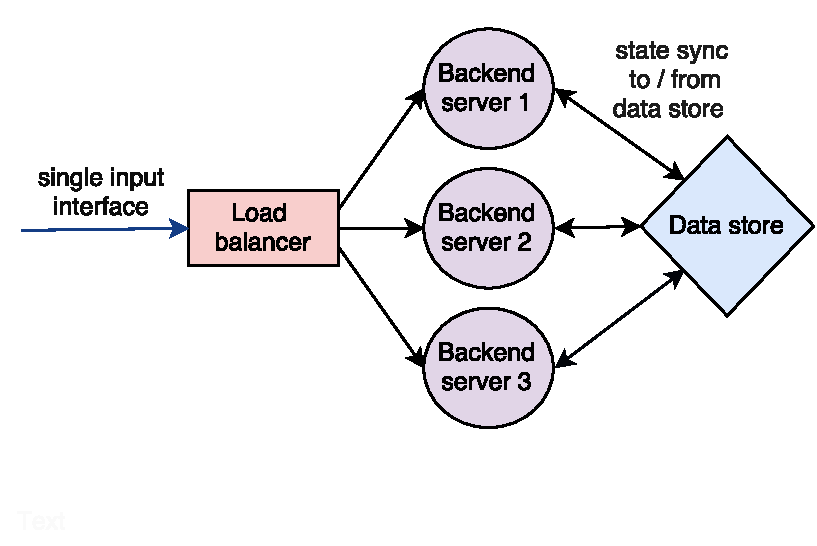
\includegraphics[scale=0.55]{images/cluster.pdf}
\caption{Distributed architecture of single EPC component
MME / SGW / PGW}
\label{fig:singlel}
\end{figure}
To transform the monolithic design of v1.0 to a scalable one, we need to replace the monolithic EPC components with a distributed version. Figure \ref{fig:singlel} shows such a distributed-cluster for our EPC elements. In this design, components namely MME, SGW and PGW are replaced by clusters consisting of a load balancer, a shared data store and a number of back-end worker servers. The overall architecture of the scalable EPC with distributed clusters in place of monolithic VNFs is shown in Figure \ref{fig:overall}. Control-plane path has been highlighted in blue and data-plane in red. This shows how each VNF cluster interfaces with other VNF components of the LTE EPC system. 
\begin{figure}
\centering
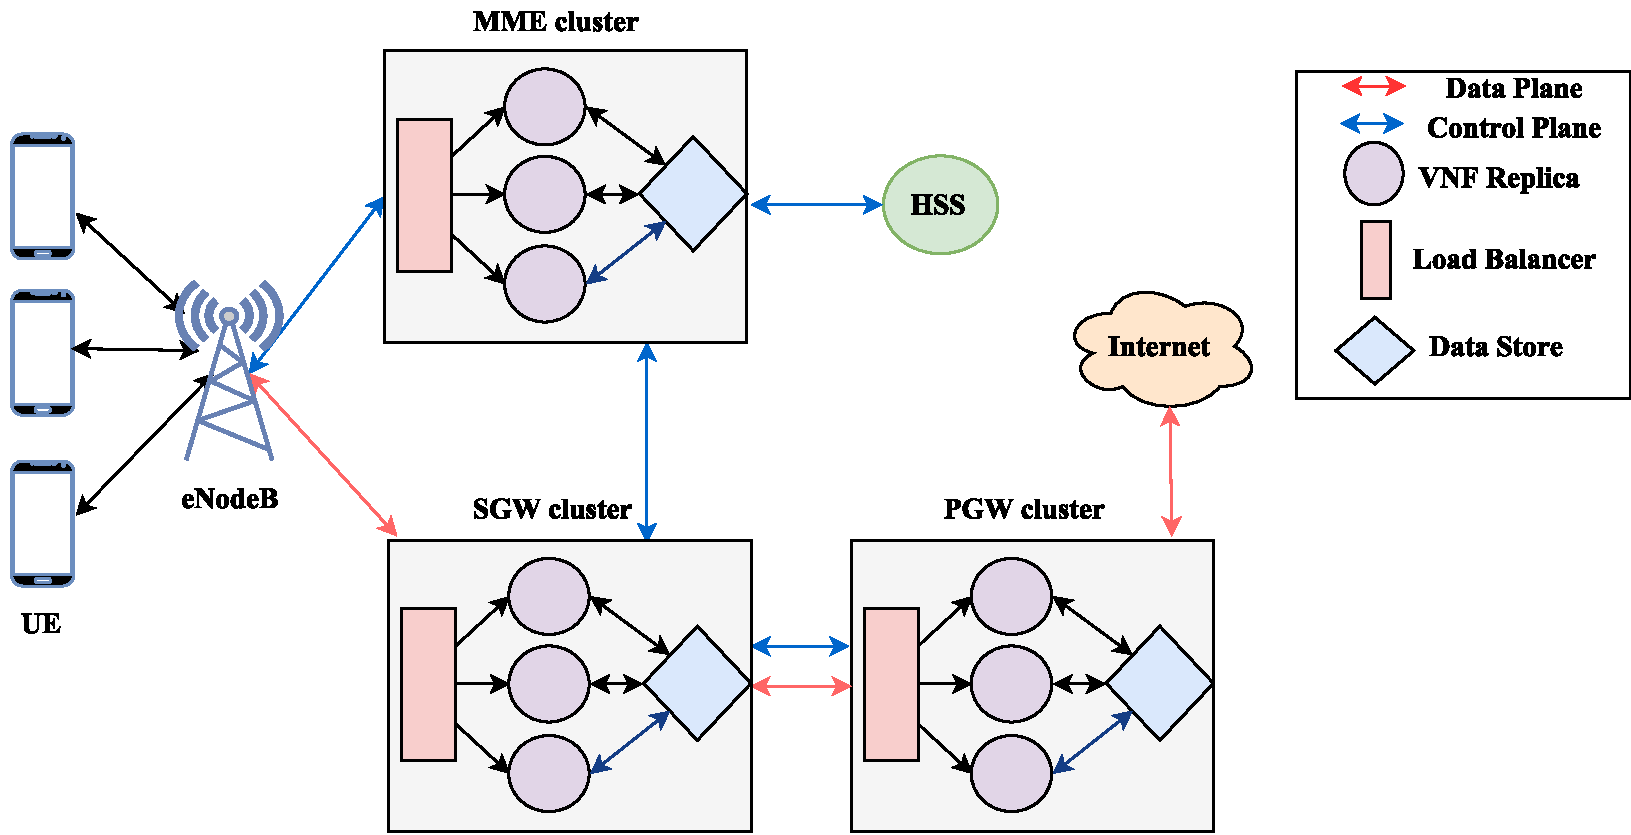
\includegraphics[scale=0.45]{images/depc.pdf}
\caption{The complete distributed LTE EPC architecture for a three worker system}
\label{fig:overall}
\end{figure}

\section*{Different state synchronization paradigms in LTE EPC}

\par A working EPC involves some permanent states (user's subscriber information) and some transient states (tunnel identifiers) which lasts only till the user is Attached. All states involved are UE centric i.e they can be represented in a key value pair with user identifier as the key. EPC VNFs use a shared key value store  for storing/retrieving the user states (referred as state synchronization here onwards). State synchronization  involves creating and updating UE state in the data store in control plane and fetching the UE state information back in data plane. As an example, in Attach operation some UE states are created and pushed to data store at S/P-GWs and in data plane these forwarding states are read back to forward user's data packets. This user state can also be kept at another sibling replica instead of the data store as one more design variant.

\par We now describe the three design options for state synchronization. 


\noindent\textbf{No sync:}

We consider the extreme case where the distributed EPC need not have any shared data store. All UE state are local to the replica in a state partitioned manner. A particular MME, S/P-GW replica handle the request of a particular UE. To achieve this the load balancer must be aware of the static mapping of UE to the particular replica of MME and S/P-GW that is responsible for keeping its state. This can be done by hashing the UE identifier to obtain the replica identifier.


\begin{figure}[H]
\centering
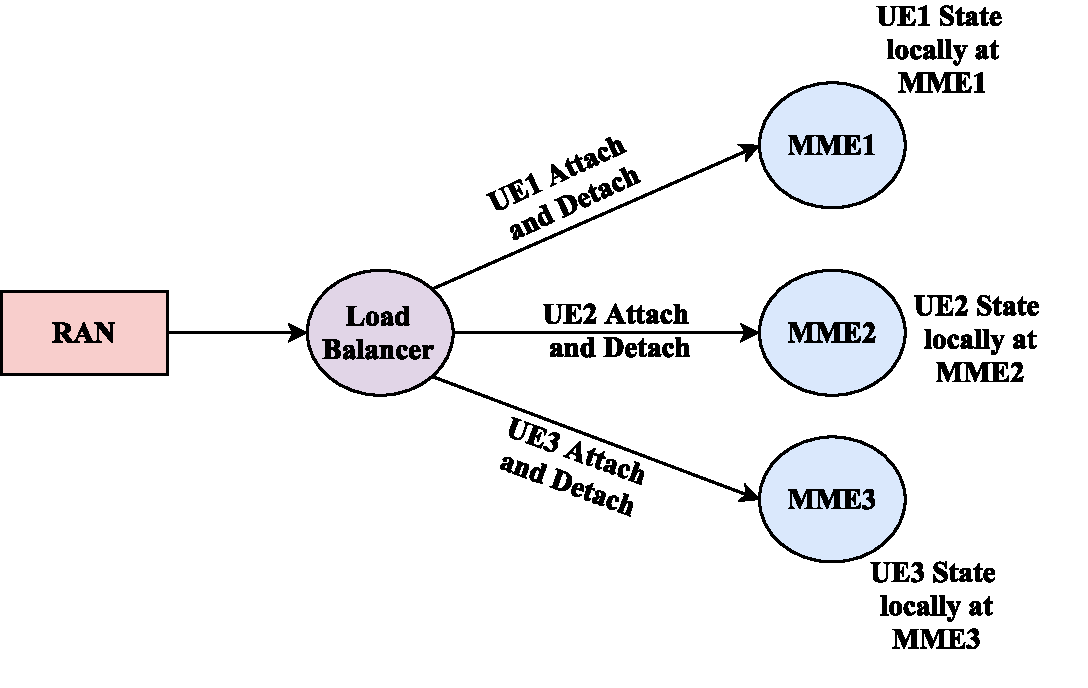
\includegraphics[scale=0.45]{images/stateful.pdf}
\caption{No sync mode for a 3 worker distributed EPC}
\label{fig:nosync}
\end{figure}
 Although this design option has no state synchronization overhead, it under-performs in terms of fault tolerance. Once a replica goes down, the state information associated with it is also lost and the user has to perform an Attach/Reattach to proceed incurring a significant overhead. As an illustration, Figure \ref{fig:nosync} shows the distributed MME cluster with no state synchronization. We can see that both Attach and Detach procedure of a particular UE are handled by the same MME replica. The same design approach is used for Attach and Detach operations at S/P-GW. 
 
 
\begin{figure}[H]
\centering
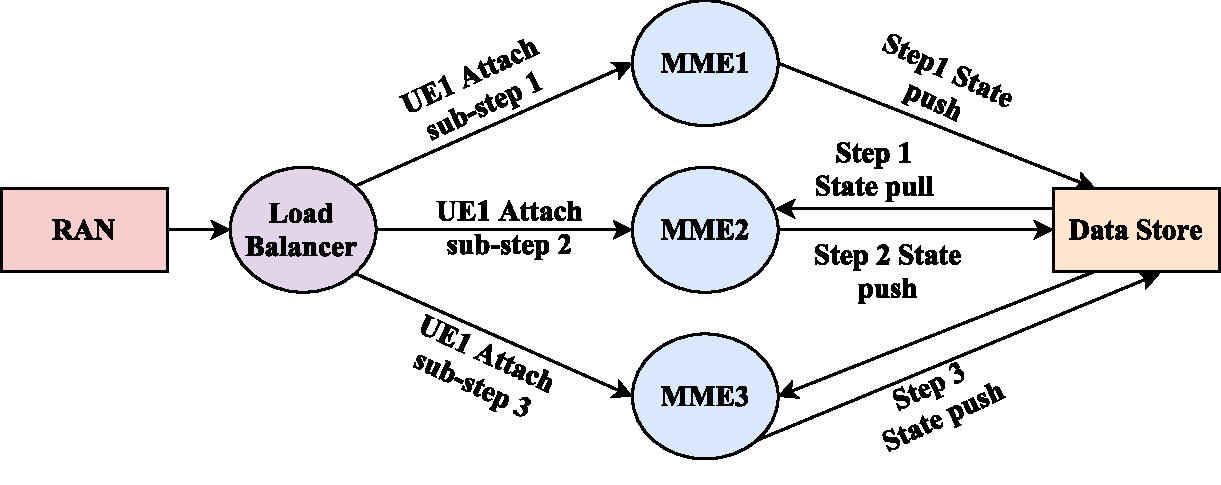
\includegraphics[scale=0.45]{images/stateless.pdf}
\caption{Always sync mode for a 3 worker distributed EPC}
\label{fig:alsync}
\end{figure}
\noindent\textbf{Always sync:}

The next design option we discuss captures the other extreme of state synchronization frequency. Here we perform state synchronization at the end of each message making the replicas completely stateless. The load balancer need not store any specific mapping as any message can be sent to any of the replicas. Figure \ref{fig:alsync} shows the scenario where each message of an Attach procedure can be routed to any of the MME replicas. After processing a message the replica must push the state information to the shared data store. When another replica receives the next message from the particular UE, it fetches the last synced state information from the shared data store and continues with the processing of further incoming messages. In terms  of fault tolerance, this system performs better than previous as failure between any multi-step user request can be tolerated and another replica can continue from where the offline replica left out.  


%\begin{center}
\begin{figure}[H]
\centering
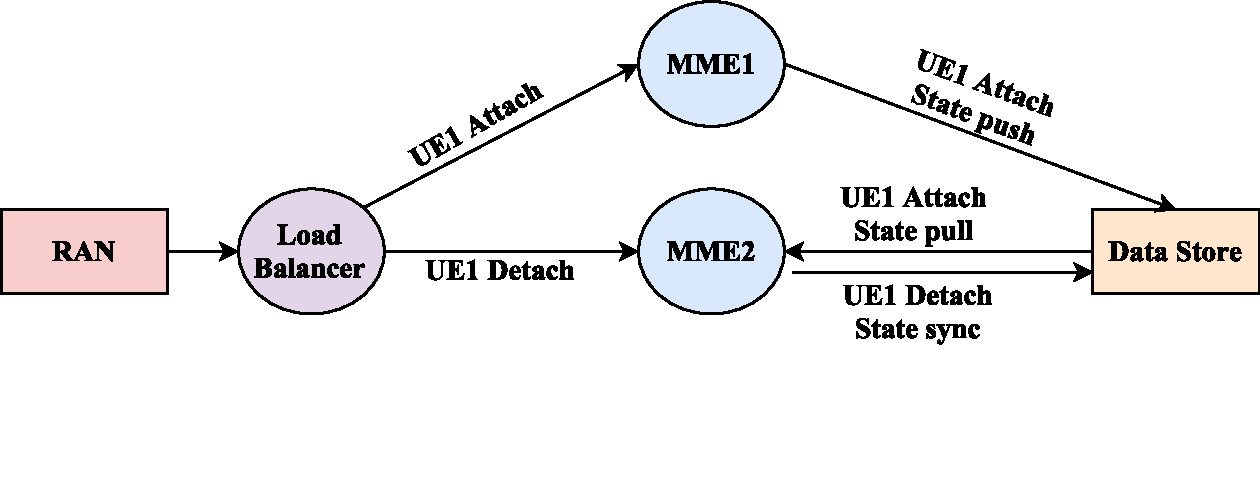
\includegraphics[scale=0.45]{images/session.pdf}
\caption{Session sync mode for a 3 worker distributed EPC}
\label{fig:sessync}
\end{figure}
\noindent\textbf{Session sync}

\par As a middle-ground design of the above two choices we can choose to reduce the frequency  at which UE state is synchronized with the data store. We define a session to be  logically correlated messages from the user. As an example the consecutive steps of an Attach message or data packets of a user's data session. The idea is to keep the UE state in the replica till the end of the session and push it back to data store when the session completes. The next session can retrieve the proceedings of the last session and continue processing. The load balancer must maintain some mapping to direct messages from a particular session to the same replica. Figure \ref{fig:sessync} illustrates the scenario where all messages from User Attach session are directed to the same MME. Post session completion, the state is pushed into the data store. All detach session messages are directed to the second MME. The second MME retrieves the Attach session state from the data store and continues with the Detach operation. Similarly in data plane, the load balancer takes care of the packet affinity to a gateway (S/P-GW) replica. When the first packet arrives, the replica retrieves user state of the UE from the shared data store and keeps it in the cache. Subsequent packets get routed to the same replicas by the load balancer (using the UE to replica identifier hash) and the cached copy of the forwarding state is reused for forwarding.

\par We provide the implementation details in chapter \ref{sec:imp}. We provide a detailed discussion on quantification of performance penalties and fault tolerance in section \ref{ch4} 

\section*{Design of load-balancers}
Each cluster (MME/SGW/PGW) contains a load-balancer as a front end element which acts as an interface to the other EPC components. The primary purpose of the load-balancer is to distribute the incoming traffic to the worker nodes. Configurations in the load balancers also helps us to maintain UE and session level affinity discussed in section \ref{ch3} design options.
\subsubsection{Choice of load balancer:}
The major classes of load balancers are divided into (1) Layer-4 load balancing (performs balancing using layer 3/4 protocols) and (2) Level-7 load balancing (performs load balancing on the basis of application layer protocols and application data). As a layer-4 load balancer is faster than a layer-7 load balancer and capable enough to achieve all of our design requirements we chose to use a layer-4 load balancer for our system.

We chose the Linux virtual server (LVS) layer 4 load balancer as it has pre-configured load balancing algorithms and it is already part of the stable release of Linux kernel. Addition of newer load balancing algorithm to it can be easily done by inserting new kernel modules.

\par The LVS load balancer operates in 3 modes:

\begin{enumerate}
\item 
LVS-NAT : Works on the principle of s-nating and d-nating each incoming and outgoing packet. 
\item
LVS-TUN : Works on the principles of ip-in-ip tunneling. 
\item
LVS-DR : This is a direct return method of load balancing where the incoming traffic gets distributed to workers via the load-balancer but gets directly returned to the client by-passing the load-balancer. 
\end{enumerate}
\par LVS-DR mode provides better performance and less chance of overloading the load balancer so we chose the LVS-DR mode as our desired configuration. The LVS-DR mode has the limitation that the back-end servers should be present on the same LAN segment as of the Load-balancer node.




\noindent\textbf{How LVS-DR works:}
%\begin{center}
\begin{figure}[H]	
\centering
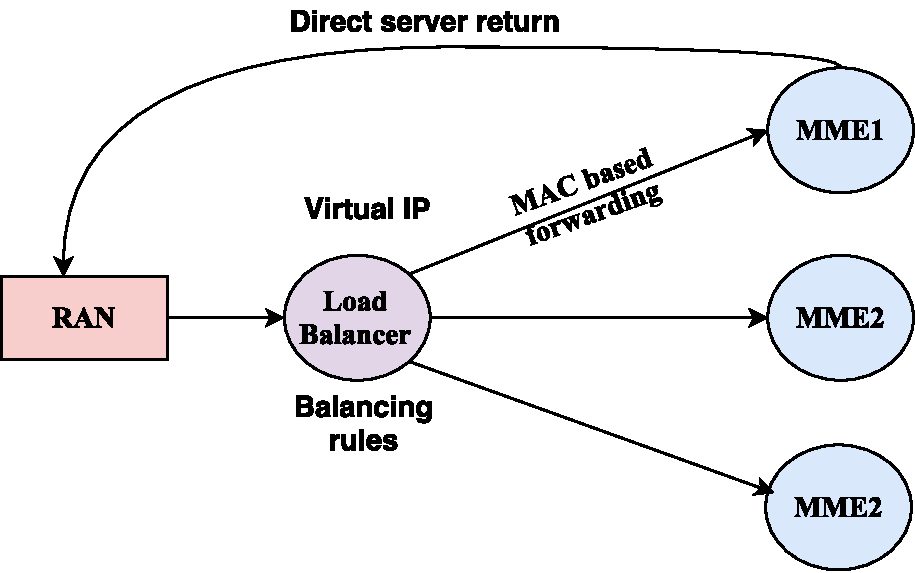
\includegraphics[scale= 0.65]{images/lvs.pdf}
\caption{A typical LVS-DR setup}
\label{fig:lbi}
\end{figure}
Figure \ref{fig:lbi} shows a typical LVS-DR setup. The setup consists of a load balancer otherwise called as director and some back-end servers. This director serves as an interface to incoming clients. The load balancer uses an ip other than its real ip also known as VIP (Virtual IP) which is exposed to clients. Load balancing rules and algorithm are configured on the director using IPVS administrator module. Once a packet reaches the director, it gets routed to one of the back-end servers via MAC based forwarding. As the packet still has the destination address of VIP and not that of the back-end servers, it has to be force consumed at the back-end server using iptables self redirect. The source address of the packet is still unchanged so the reply follows a path directly to that particular client, by-passing the director module.\\


\noindent\textbf{Failure detection and tolerance:}

For correct operation of an LVS based load balancer the offline backend server entry needs to be removed from the LB rule set. The cluster needs to know about the  online/offline status of each of the backend servers. This status can be known by a simple heatbeat message from the backend servers to the load balancer using the keepalived LVS extension. To recover from these failures the simulated UE retries the previous procedure step (e.g. authentication/setting eps step in an Attach session) for a fixed number of time. In case that fails, the whole EPC session (Attach/Detach) is retried. Figure \ref{fig:sss} demonstrates the synchronization points in all these state synchronization modes. We could see that we have to retry from the last saved checkpoint(last state synchronization point) to recover from a failure.

\begin{figure}[H]	
\centering
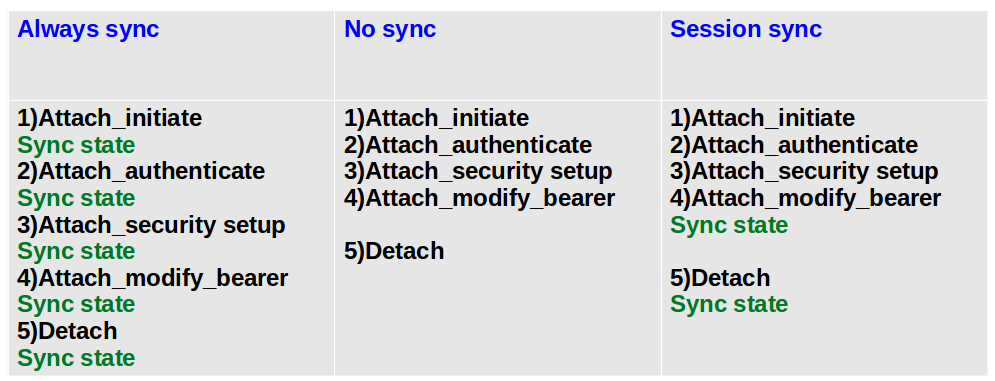
\includegraphics[scale= 0.39]{images/sync_designs.png}
\caption{State synchronization summary}
\label{fig:sss}
\end{figure}

\section*{IMPLEMENTATION}
\label{sec:imp}
As per the design outlines presented we have made required changes to NFV\_LTE\_EPC 1.0 by converting the MME S/P-GW VNFs into a clustered system. We describe the implementation details of each component in this section.

%Load balancer impl
\section*{Load balancer integration and fault tolerance in NFV\_LTE\_EPC 2.0:}

We modified each of the EPC VNFs to have a load balancer as the front end. All incoming traffic to that EPC has to pass through the front end load balancer. The load balancer is assigned with a virtual IP which will act as the visible IP to other EPC components. The load balancer can be setup in two modes (i) Round robin, where it does not have to keep any UE to replica mapping information and can route messages to any of the replica. (ii) Source hash, where the destination replicas are chosen based on the hash of the source IP:PORT pair and this mapping of hashed source to replica identifier are stored at the load balancer. These two modes of operation of the load balancer were used to achieve  desired replica affinity in the three state  synchronization modes. 
\par To ensure fault tolerance we used the keepalived extension to the LVS to monitor the heartbeat messages from the backend replicas. Once the LVS detects absence of heartbeats from a replica it removes the same entry from the load balancer. Subsequent requests targeted to the off-line replica will now get re-routed to a live one. In control plane operations \textbf{No sync} mode can not tolerate failures as all states are local. Hence it has to retry the full procedure. In \textbf{Session sync} mode once a UE completes a session, failure of that replica will not affect the overall operation. UE can simply retry only the session which failed before completion.
In \textbf{Always sync} mode all UE state is preserved after processing of each message. Hence only retrying that particular failed message will suffice to complete the remaining operation.

When a failure is simulated UEs detect the broken connection and retry for that particular failed procedure. On crossing the retry limit the horizon of retry is increases to session level. The whole Attach/Detach session is then retried for the UE. 

In addition to that to prevent the load balancer from being a single point of failure, a back up load balancer with same virtual IP can be kept in parallel. The back up can take over load balancing when the primary fails.
\section*{State separation using a shared data store:}

As discussed in earlier sections, MME and S/P-GW clusters should be stateless workers in order to scale horizontally. This requires a shared data store (key-value store) in each of these clusters. Therefore, each of the EPC VNFs was modified to keep the user state in a shared data store periodically based on the synchronization mode used.

\par In control plane operation of LTE EPC the saved states are pushed periodically to the shared datastore. This enables any back-end workers in the cluster to service a particular UE. In data plane operation the UE context information is safely present in the shared datastore. When a UE sends data packets to SGW worker, the worker can pull the UE context from shared data store and perform packet forwarding.

\par The NFV-LTE-EPC 2.0 system was integrated to key value data stores using the  intermediate API (part of the vEPC 2.0 source) that provides interfacing to various key value stores.

\section*{Implementation changes at EPC VNF replicas}

We made minor changes to the EPC VNF replicas in order to accommodate for the load balancer as the front end entity. Similarly we had to make changes to the state synchronization logic to serialize and push the user state into the data store. The front end load balancers and the shared data store integration ensured scalability, stateless properties and fault tolerance. 

\par For exploring the three design options of state synchronization we modified the way VNFs synchronize user states in the following way. 

For \textbf{Always sync} mode the load balancer is at liberty to send packet to any of the replicas of a particular VNF. The load balancer is set to round robin load balancing mode as it does not have the responsibility to store any mapping. The replica synchronizes user states after processing of every message.

For \textbf{No sync} mode the load balancer must send the packets of a particular UE to a particular replica. As an illustration, to facilitate this at the SGW replicas, the load balancer at the front end must be configured in source hash mode. The MME replica must use the same socket(IP-Port pair) for forwarding the packets of a particular UE. For No sync mode (where both Attach and Detach must go to the same replica) MME must keep on using the same socket for both Attach and Detach procedure by identifying packets based on their tunnel identifier.

For \textbf{Session sync} mode the load balancer must send the packets of a particular UE to a particular replica only until the end of session boundaries(e.g. end of Attach / Detach session or user data session). Similar to the previous design, the load balancer at the front end must be configured in source hash mode. To facilitate this at SGW replicas  the MME replica must use the same socket(IP-Port pair) for forwarding. For Session sync mode (where only Attach or Detach must go to the same replica) MME can segregate packets based on their tunnel id (UE identifier) and keep on using the same socket till the end of that session.

The three synchronization modes discussed were similarly used for other EPC VNFs in control plane to achieve the desires design specification.

%\begin{center}
\begin{figure}[H]
\centering
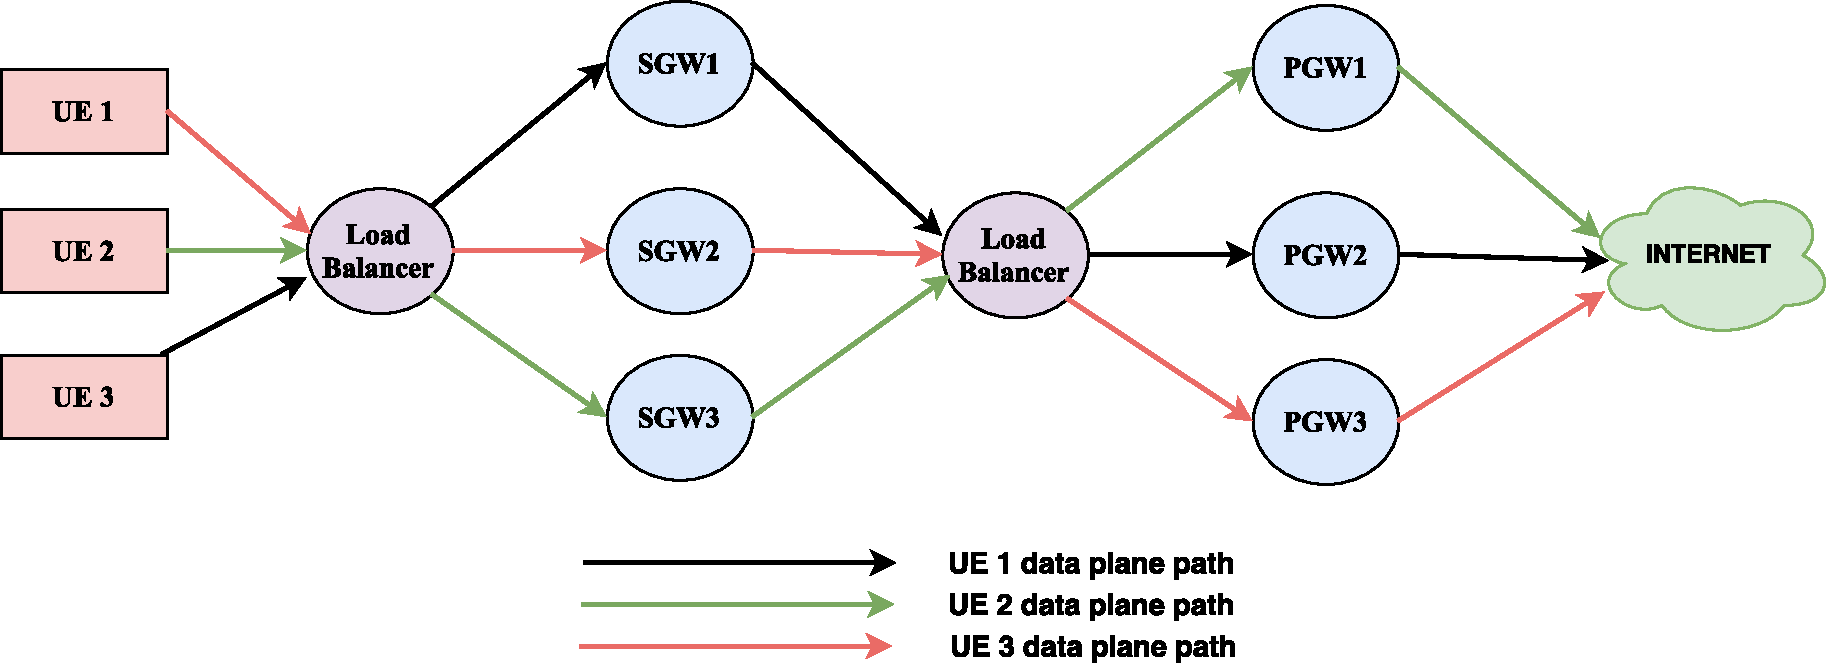
\includegraphics[width = \linewidth]{images/datapath.pdf}
\caption{UE data packet flow illustration}
\label{fig:dpath}
\end{figure}
\par The same implementation has been followed  in data plane for up/down link traffic. Each of the previous VNFs ensures to use same socket over the session for sending data packets of the same UE. Figure \ref{fig:dpath} shows a possible flow of packets of three UE groups. We can see that in this scenario packets of a particular UE group (Group 1) always travels through replica 1 of SGW, and replica 2 of PGW to ensure reuse of the cached forwarding state.\\
%shared data store

More clarity on the implementation can be achieved by going through the in-code documentation and usermanual provided.
Future work in this area can be to integrate with some kernel bypass mechanism to increase the data plane performance.

\end{document}